\documentclass[11pt]{article}
\usepackage{amsmath,textcomp,amssymb,geometry,graphicx,rotating,multirow, listings}

\lstset{breaklines=true}

\def\Name{Sahar Mesri, Sagar Karandikar}
\def\Login{cs150-bw, cs150-bn}

\title{CS150 Checkpoint 3 Proposal, Team 07}
\author{\Name, \texttt{\Login}}
\pagestyle{myheadings}

\begin{document}
\maketitle
\section*{1. Block Diagrams}

\subsection*{Overall System}

\noindent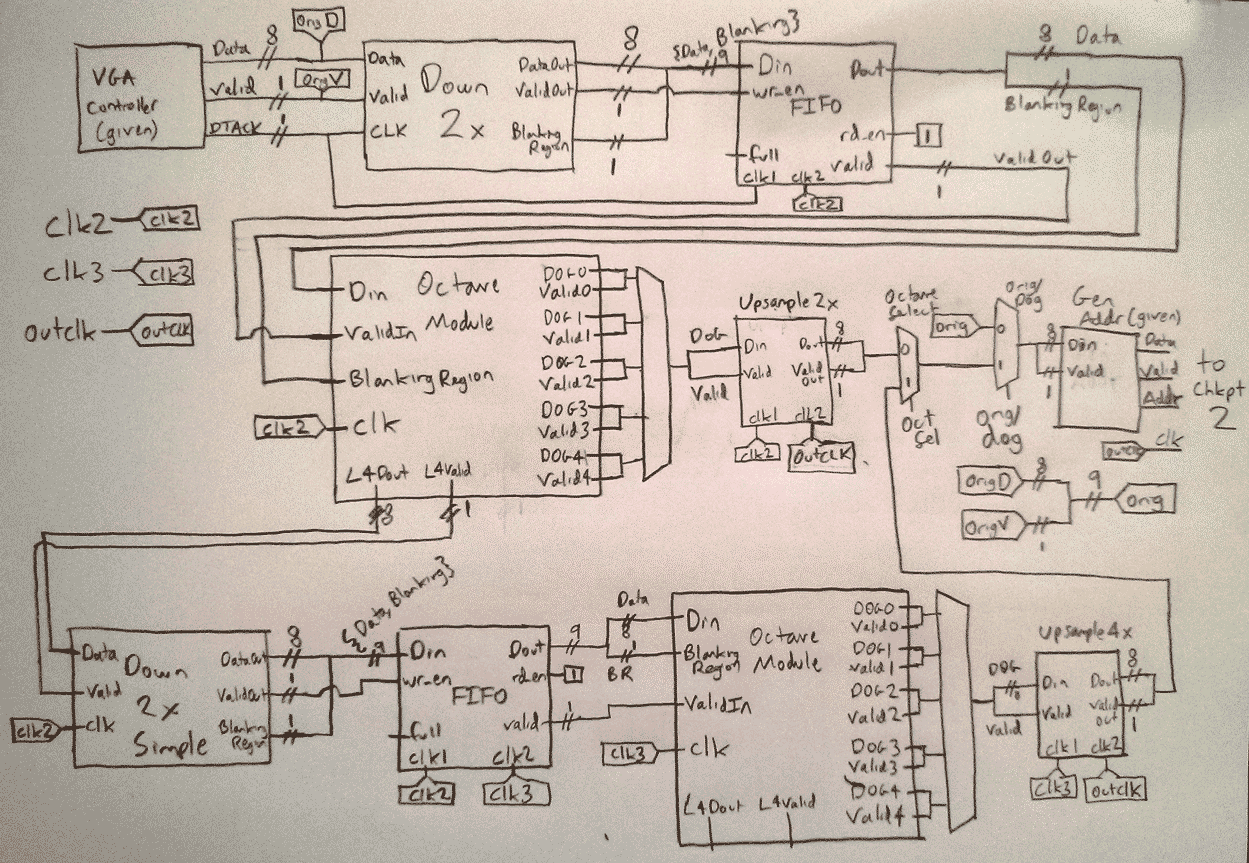
\includegraphics[width=\textwidth]{modules/procoverall.png}

\newpage

\subsection*{a. Gaussian Filter Banks}

Octave Module:

Delay blocks are 2112 byte wide shift registers. \newline


\noindent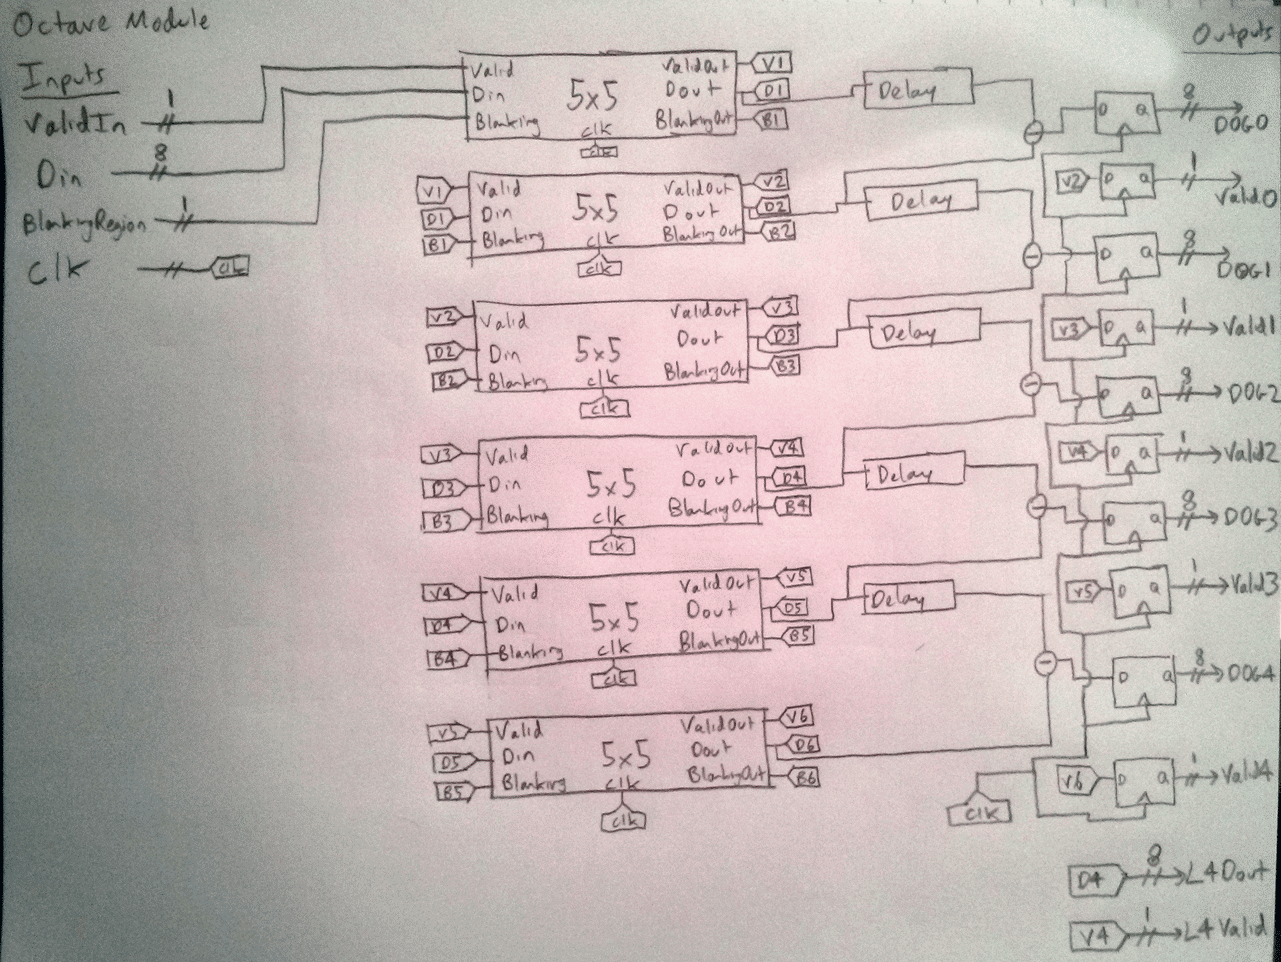
\includegraphics[width=\textwidth]{modules/prococtave.png}

\newpage

5x5 Window Module:

Delay block is a 2112 bit wide shift register or a 1062 bit wide shift register (corresponding to 420 pixels wide and 210 pixels wide respectively). \newline

\noindent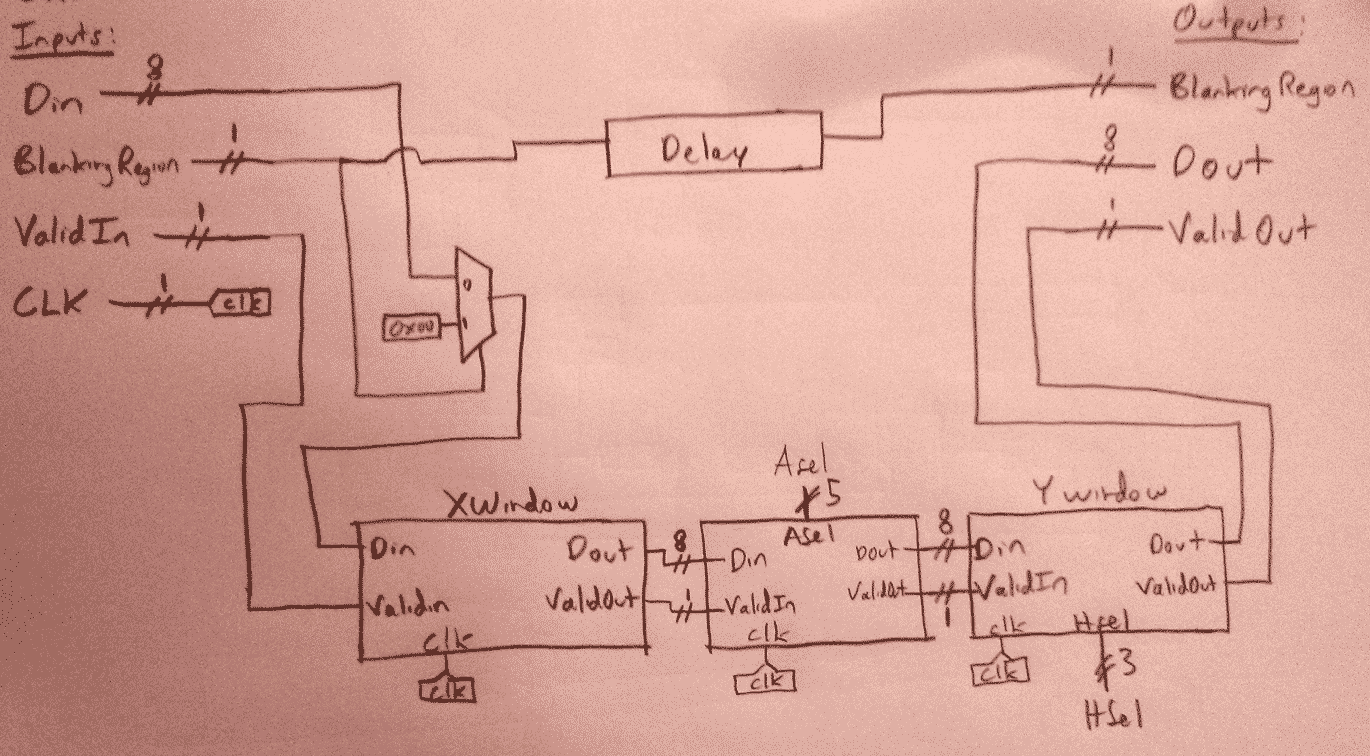
\includegraphics[width=\textwidth]{modules/proc5x5window.png}

\newpage
X Window Module:

Data lines after multiplication blocks are all 16 bits wide, DOUT is cut
back down to 8 bits. \newline

\noindent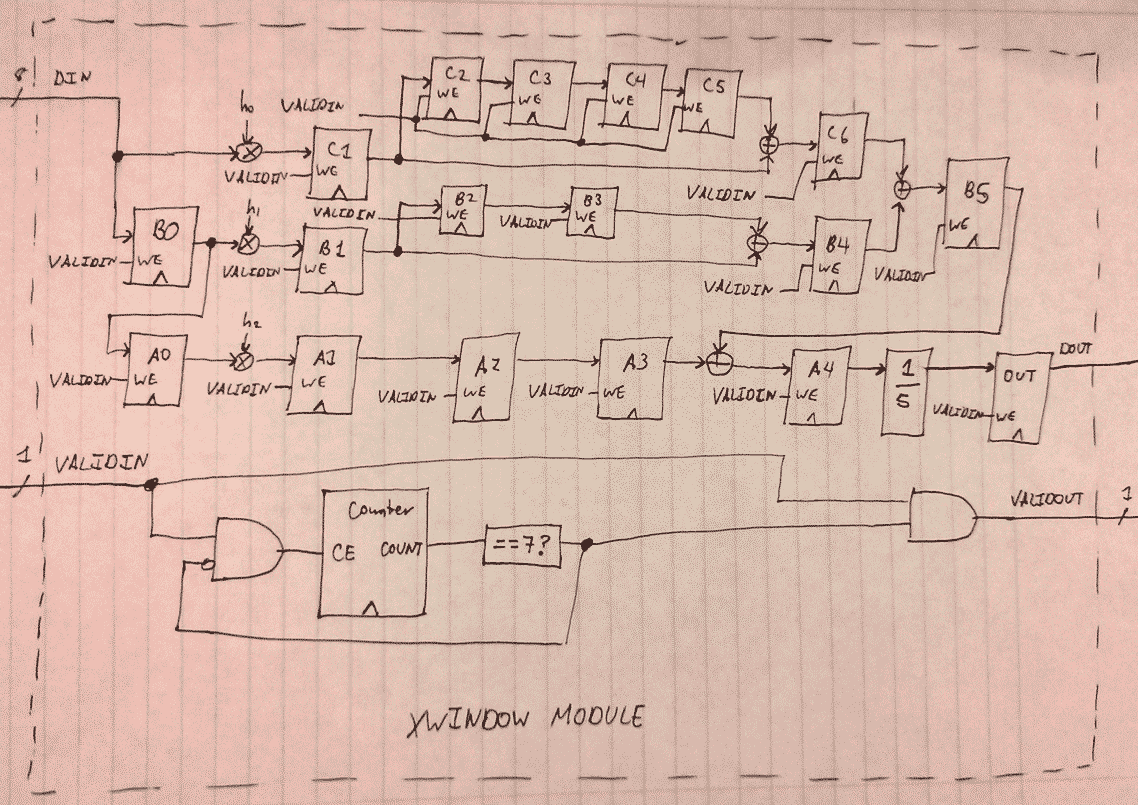
\includegraphics[width=\textwidth]{modules/procx_window.png}

\newpage 

Y Window Module:

Data lines after multiplication blocks are all 16 bits wide, DOUT is cut
back down to 8 bits. \newline

\noindent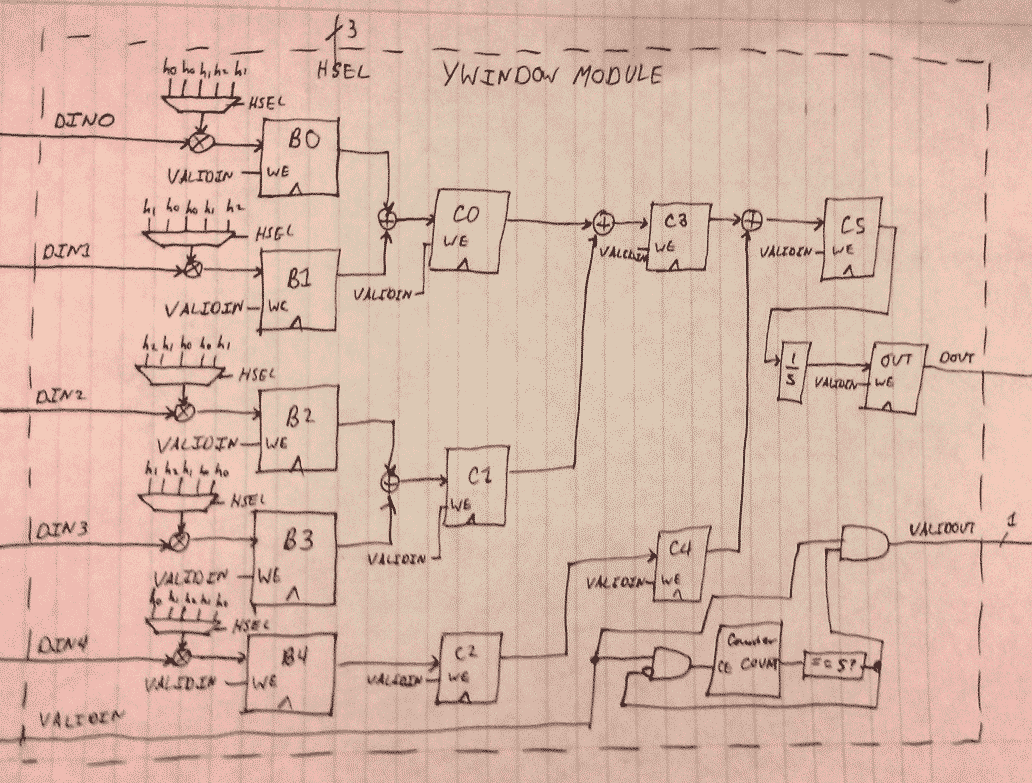
\includegraphics[width=\textwidth]{modules/procy_window.png}

\newpage

5 Row Array Module:

Shift registers are 420 bytes wide or 210 bytes wide. \newline

\noindent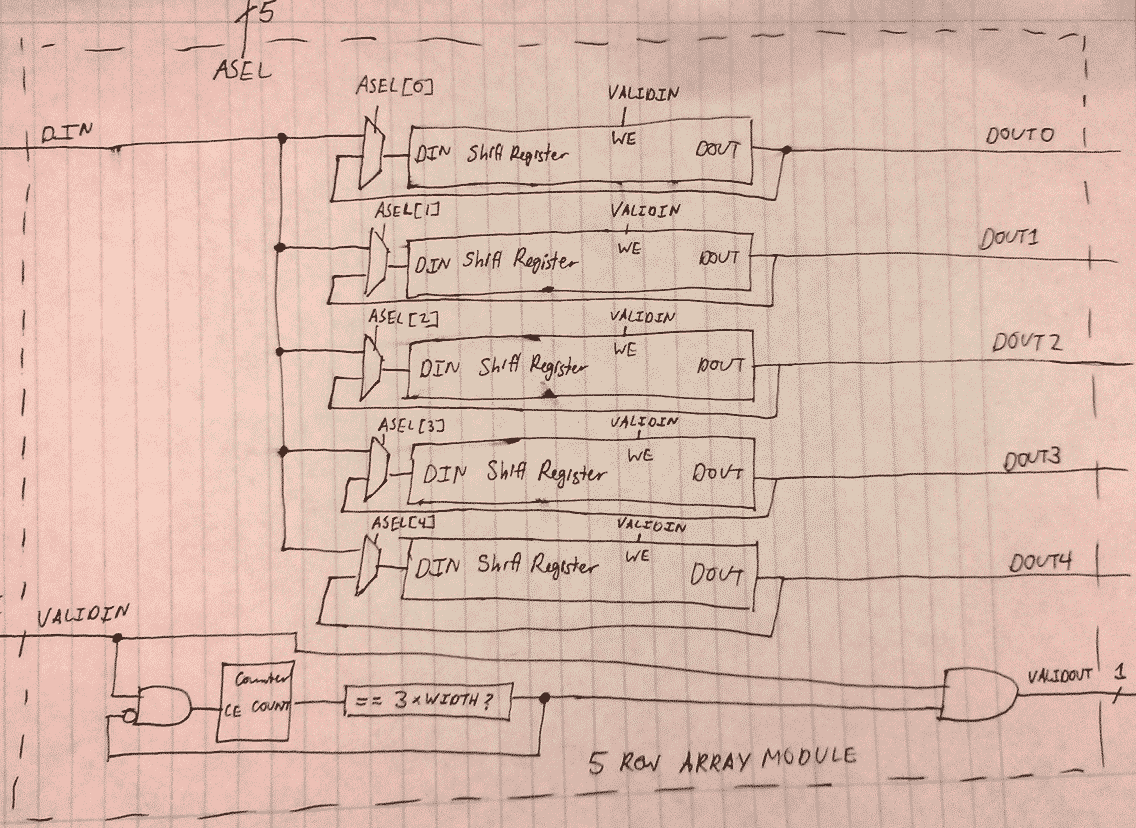
\includegraphics[width=\textwidth]{modules/proc5row.png}

\newpage

\subsection*{b. Downsampling}

800x600 to 420x320 downsampler (2x + adds padding): \newline

\noindent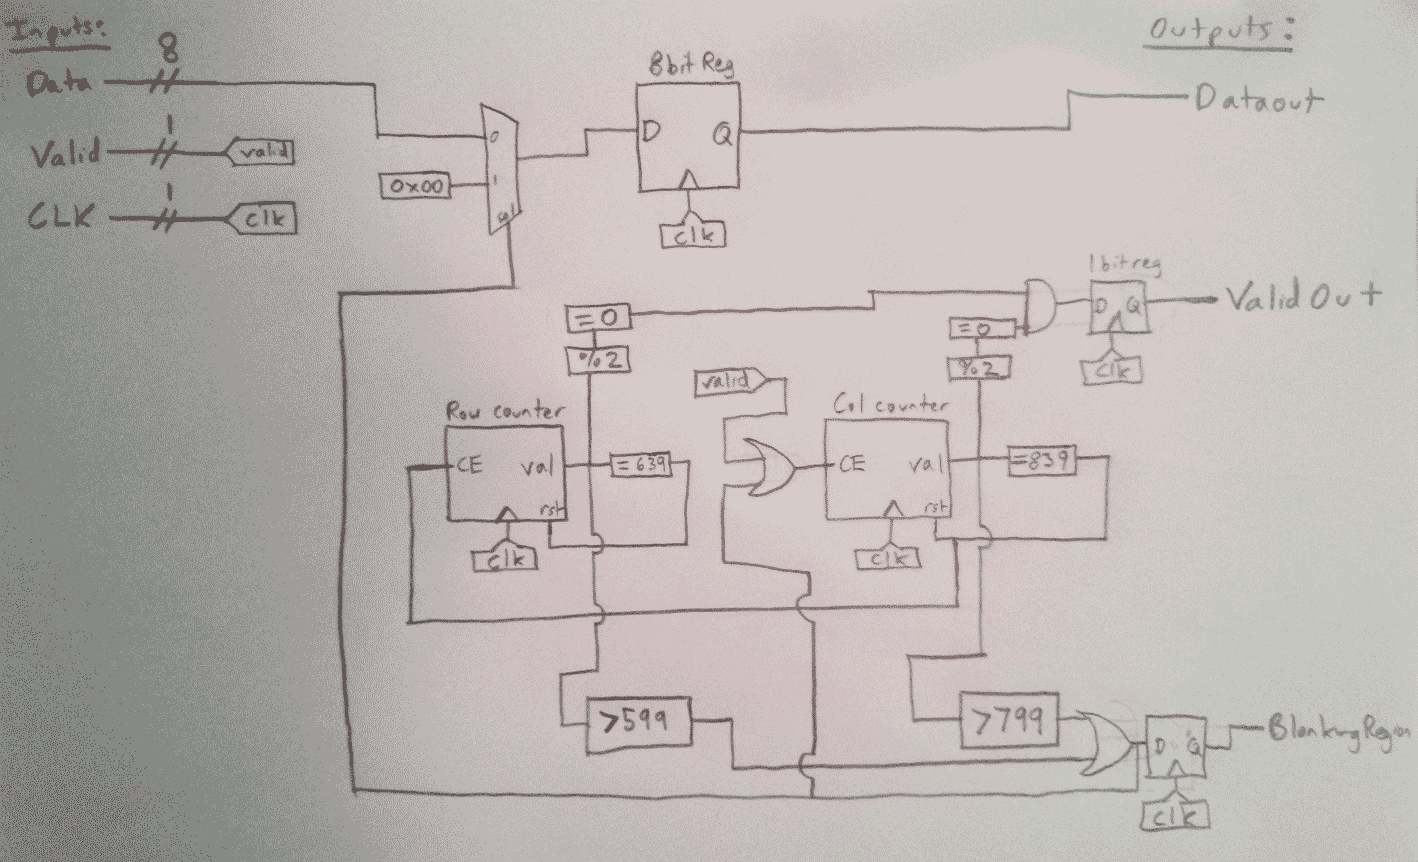
\includegraphics[width=\textwidth]{modules/procdownsampler2x.png}

\newpage

\noindent 420x320 to 210x160 downsampler (2x) \newline

\noindent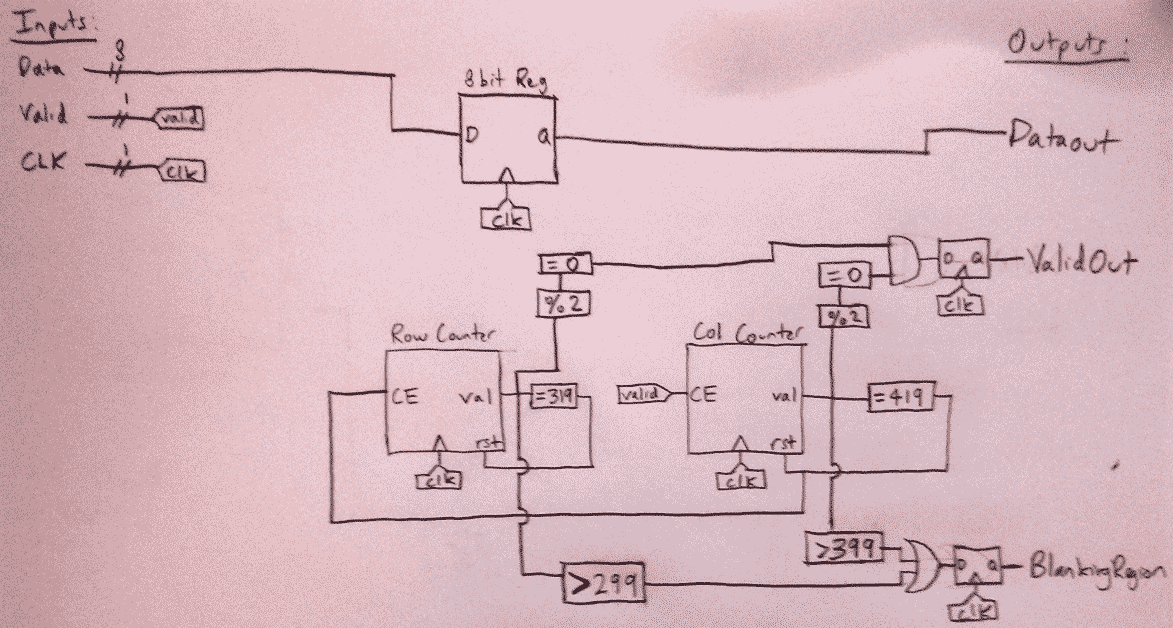
\includegraphics[width=\textwidth]{modules/procdownsampler2x_simple.png}

\newpage

\subsection*{c. Upsampling}

\noindent Upsample 2x: \newline

\noindent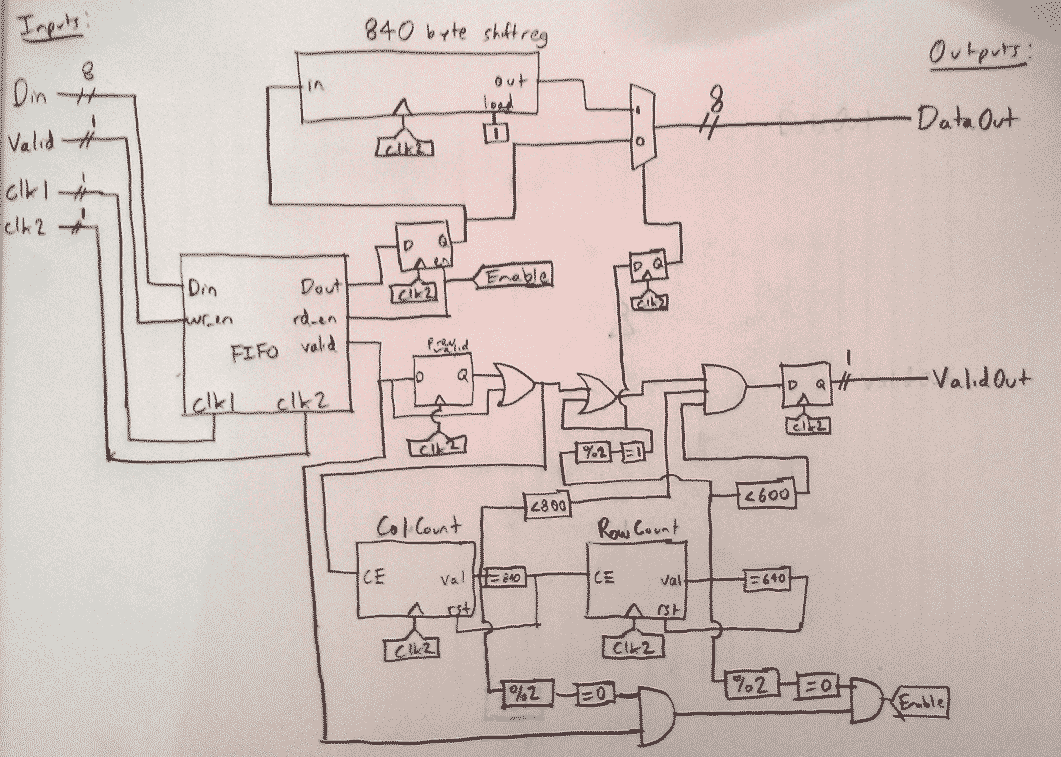
\includegraphics[width=\textwidth]{modules/procupsample2x.png}

\newpage

\noindent Upsample 4x: \newline

\noindent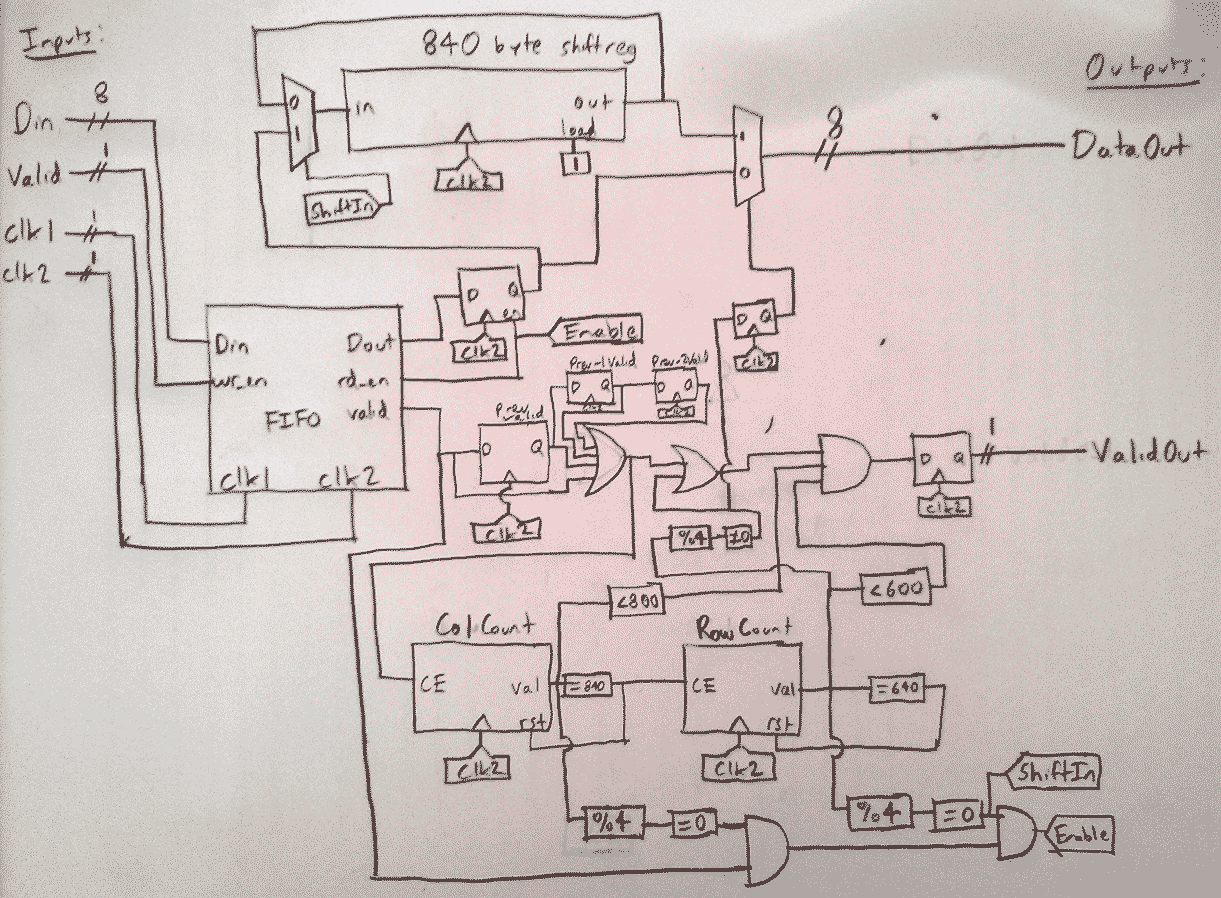
\includegraphics[width=\textwidth]{modules/procupsample4x.png}

\subsection*{d. Interface Connections}

(See overall diagram)

\section*{2. List of Signals}

\subsection*{Datapath Inputs}

\indent8 bit Data In (from VGA controller)

1 bit Valid  (from VGA controller)

1 bit DTACK (from VGA controller)

3 external clocks (not necessarily different clocks, but can be to reduce stalls)

1 bit out\_sel: selects which octave to output if orig/dog = dog

1 bit orig/dog: 0 indicates output VGA input, 1 indicates output dog octave indicated by out\_sel

5 bit ASEL into 5 Row Array Module

3 bit HSEL into Y Window Module

\subsection*{Datapath Outputs}

8 bit Data Out

1 bit Valid Out

18 bit Address Out (from Address Generator block)

1 bit output clock (for checkpoint 2 write clock)

\section*{3. RT Language Description}

\subsection*{Octave Module}
\begin{lstlisting}
while(true){
    Dog0ShiftReg <- (D1 << 2111*8) | (Dog0ShiftReg >> 8),
    Dog1ShiftReg <- (D2 << 2111*8) | (Dog1ShiftReg >> 8),
    Dog2ShiftReg <- (D3 << 2111*8) | (Dog2ShiftReg >> 8),
    Dog3ShiftReg <- (D4 << 2111*8) | (Dog3ShiftReg >> 8),
    Dog4ShiftReg <- (D5 << 2111*8) | (Dog4ShiftReg >> 8),
    Dog0Reg <- Dog0ShiftReg - D2,
    Dog1Reg <- Dog1ShiftReg - D3,
    Dog2Reg <- Dog2ShiftReg - D4,
    Dog3Reg <- Dog3ShiftReg - D5,
    Dog4Reg <- Dog4ShiftReg - D6,
    Valid0Reg <- V2,
    Valid1Reg <- V3,
    Valid2Reg <- V4,
    Valid3Reg <- V5,
    Valid4Reg <- V6;
}
\end{lstlisting}

\subsection*{5x5 Window Module}
\begin{lstlisting}
while(true){
    DelayShiftReg <- (BlankingRegion << 2111) | (DelayShiftReg >> 1),
    XWindow Ops, 5x5 Array Ops, YWindow Ops;
}
\end{lstlisting}

\subsection*{X Window Module}
\begin{lstlisting}

while(true){
    if(ValidIn) {
        B0 <- Din, A0 <- B0, C1 <- h0*Din, B1 <- h1*B0, 
        A1 <- h2*A0, C2 <- C1, C3 <- C2, C4 <- C3, 
        C5 <- C4, C6 <- C5 + C1, B2 <- B1, B3 <- B2, 
        B4 <- B3 + B1, B5 <- C6 + B4, A2 <- A1, 
        A3 <- A2, A4 <- B5 + A3, Out <- 1/5 * A4, 
        Counter <- Counter + 1 if Counter != 7;
    }
}
\end{lstlisting}

\subsection*{Y Window Module}
\begin{lstlisting}
while(true){
    if(ValidIn){
        B0 <- coeff*DIN0, 
        B1 <- coeff*DIN1, 
        B2 <- coeff*DIN2, 
        B3 <- coeff*DIN3, 
        B4 <- coeff*DIN4, 
        C0 <- B0 + B1, C1 <- B2 + B3, 
        C2 <- B4, C3 <- C0 + C1, C4 <- C2, 
        C5 <- C3 + C4, Out <- 1/5*C5, 
        Counter = Counter + 1 if Counter != 5;
    }
}
\end{lstlisting}

\subsection*{5 Row Array Module}

\begin{lstlisting}
while(true){
    if(ValidIn){
        ShiftReg0 <- {(DIN if ASEL[0] else (ShiftReg0 & 0xFF)),  (ShiftReg0 >> 8)},
        ShiftReg1 <- {(DIN if ASEL[1] else (ShiftReg1 & 0xFF)),  (ShiftReg1 >> 8)},
        ShiftReg2 <- {(DIN if ASEL[2] else (ShiftReg2 & 0xFF)),  (ShiftReg2 >> 8)},
        ShiftReg3 <- {(DIN if ASEL[3] else (ShiftReg3 & 0xFF)),  (ShiftReg3 >> 8)},
        ShiftReg4 <- {(DIN if ASEL[4] else (ShiftReg4 & 0xFF)),  (ShiftReg4 >> 8)},
        Counter = Counter + 1 if Counter != 3*WIDTH;
    }
}
\end{lstlisting}

\subsection*{2x Downsampler}
\begin{lstlisting}
while(true){
    DataoutReg <- 0x00 if PrevBlankingRegion else Data,
    RowCounter <- RowCounter + 1 if ColCounter == 839 else RowCounter,
    ColCounter <- ColCounter + 1 if valid & PrevBlankingRegion else ColCounter,
    ValidOutReg <- ColCounter % 2 == 0 && RowCounter % 2 == 0;
}
\end{lstlisting}

\subsection*{2x Downsampler Simple}
\begin{lstlisting}
while(true){
    DataoutReg <- Data,
    RowCounter <- RowCounter + 1 if ColCounter == 419 else RowCounter,
    ColCounter <- ColCounter + 1 if valid else ColCounter,
    ValidOutReg <- ColCounter % 2 == 0 && RowCounter % 2 == 0;
}
\end{lstlisting}

\subsection*{2x Upsample}
\begin{lstlisting}
while(true){
    DoutReg <- Dout, 
    PrevValid <- valid, ColCount <- ColCount + 1 if valid or PrevValid else ColCount, 
    RowCount <- RowCount + 1 if ColCount == 840 else RowCount, 
    ValidOutReg <- (PrevValid | Valid | (RowCount % 2 == 1)) & ColCount < 800 & RowCount < 600, 
    MuxSelReg <- RowCount % 2 == 1, 
    ShiftReg <- (ShiftReg >> 8) | (DoutReg << 839*8);
}
\end{lstlisting}

\subsection*{4x Upsample}
\begin{lstlisting}
while(true){
    DoutReg <- Dout, 
    PrevValid <- valid, 
    ColCount <- ColCount + 1 if valid or PrevValid else ColCount, 
    RowCount <- RowCount + 1 if ColCount == 840 else RowCount, 
    ValidOutReg <- (PrevValid | Valid | (RowCount % 4 != 0) | Prev-1Valid | Prev-2Valid) & ColCount < 800 & RowCount < 600, 
    MuxSelReg <- RowCount % 4 != 0, ShiftReg <- (ShiftReg >> 8) | (DoutReg << 839*8) if ShiftIn else (ShiftReg >> 8) | (ShiftReg << 839*8), 
    Prev-1Valid <- PrevValid, 
    Prev-2Valid <- Prev-1Valid;
}
\end{lstlisting}


\section*{4. Controller State Diagram}

The pipeline does not have a single controller, rather each individual module
inside contains its own controller, excluding the two controllers described below. 
The controllers integrated into each module follow the following format:

\begin{itemize}
    \item[(1)] Remain in Idle until Valid is received.
    \item[(2)] Begin iterating over pixels (number of pixels depends on frame size at that point in the computation), increasing the column counter values
        by one for each valid pixel input and resetting the column counter and adding
        one to the row counter at the end of a row. In the case where the pixel
        input is not valid, the controller will remain in the last state.
    \item[(3)] Upon completion return to idle (counters set to 0, 0), wait for next valid signal (in idle).
\end{itemize}

\subsection*{ASel controller for 5x5 Array}

\noindent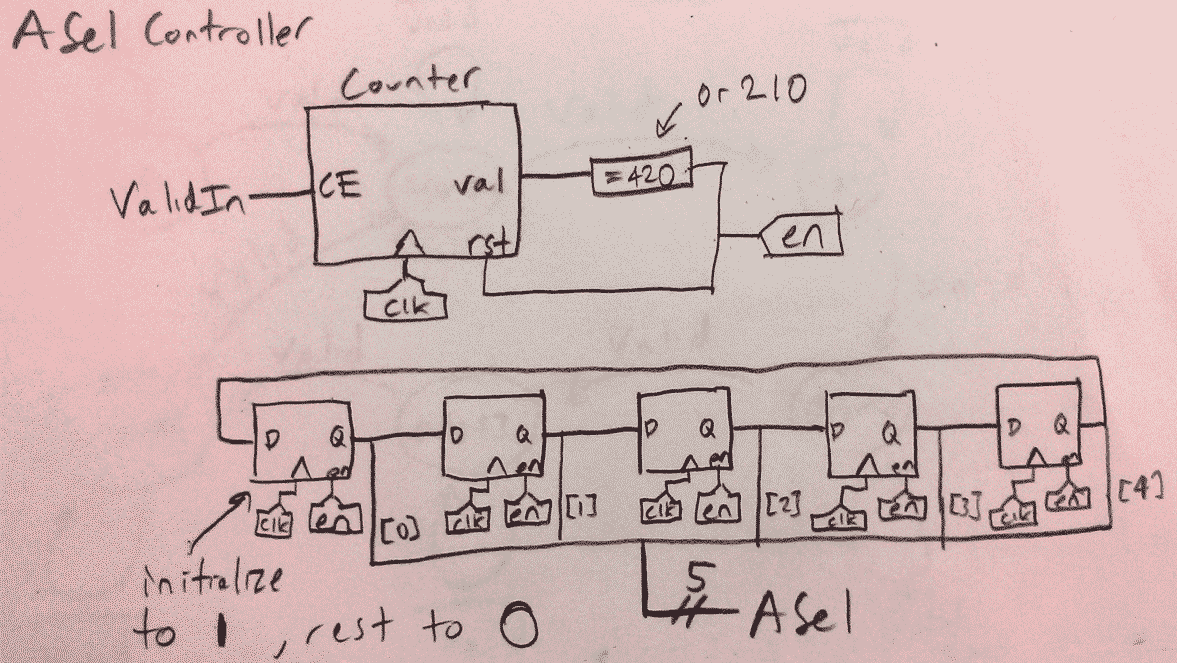
\includegraphics[width=\textwidth]{controllers/procasel.png}

\subsection*{HSel controller for Y window}

\noindent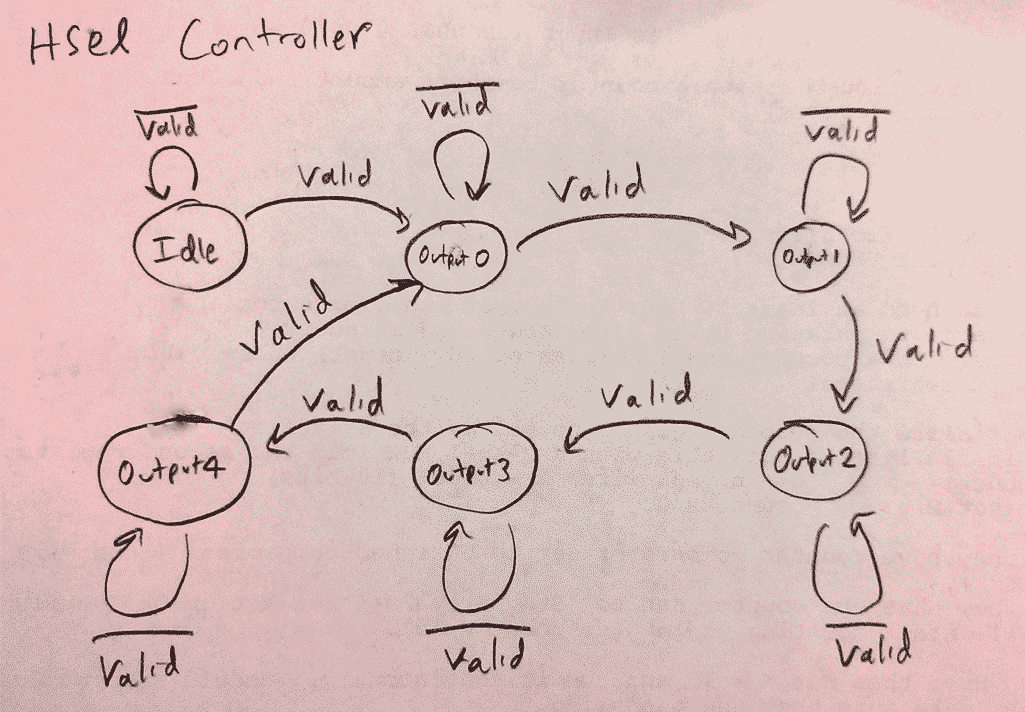
\includegraphics[width=\textwidth]{controllers/prochsel.png}

\section*{5. Testbench Outline}
Overall System:
\begin{itemize}
    \item Feed in 800x600 pixel image, simulating inputs from VGA controller, check that outputs are correct DoG.
    \item Output correctness can be tested using existing python script.
\end{itemize}

\noindent Octave Module:
\begin{itemize}
    \item Feed in 5x5 window of data, confirm that 5 DoGs are computed correctly.
    \item Potential failure modes:
        \begin{itemize}
            \item Delay length for alignment of DoG computation.
            \item Reacting to deassertion of validIn.
            \item Ensure correct valid signal propagation for display.
        \end{itemize}
\end{itemize}


\noindent 5x5 Window Module:
\begin{itemize}
    \item Feed in 5x5 window of data, confirm 2D convolution output.
    \item Potential failure modes:
        \begin{itemize}
            \item Correct coefficient selection (FSM will go here).
            \item Delay length for BlankingRegion.
            \item Reacting to deassertion of validIn.
            \item Ensure correct handling of BlankingRegion (should force input to zero in the region).
        \end{itemize}
\end{itemize}


\noindent X Window Module:
\begin{itemize}
    \item Feed in row at a time of video signal and confirm horizontal convolution output.
    \item Potential failure modes:
        \begin{itemize}
            \item Correct coefficient selection.
        \end{itemize}
\end{itemize}


\noindent Y Window Module:
\begin{itemize}
    \item Feed in column at a time of video signal (columns that are 5 pixels tall) and confirm vertical convolution output.
    \item Potential failure modes:
        \begin{itemize}
            \item Correct coefficient selection.
        \end{itemize}
\end{itemize}


\noindent 5 Row Array Module:
\begin{itemize}
    \item Feed in first 5 lines of 420x320 AND 210x160 signal, should receive one ``column'' out per cycle, consisting of 5 elements. This should continue for 420 cycles for 420x320 and 210 cycles for 210x160.
    \item Potential failure modes:
        \begin{itemize}
            \item Reacting to Valid going low (potential for incorrect values to enter shift registers?).
        \end{itemize}
\end{itemize}


\noindent 800x600 to 420x320 downsampler (2x + adds padding):
\begin{itemize}
    \item Feed in 800x600 signal, should receive 420x320 signal out
    \item Potential failure modes:
        \begin{itemize}
            \item Off by one errors in counter logic.
            \item Reacting to Valid going low.
            \item Case where pipeline consuming data much slower than VGA provides it (FIFO overflow).
            \item FIFO delay handling.
            \item Potential for errors in adding artificial blanking region.
            \item Guaranteed failure if input VGA blanking period is not at least 40px in each direction.
        \end{itemize}
\end{itemize}


\noindent 420x320 to 210x160 downsampler (2x):
\begin{itemize}
    \item Feed in 420x320 signal, should receive 210x160 signal out
    \item Potential failure modes:
        \begin{itemize}
            \item Off by one errors in counter logic.
            \item Reacting to Valid going low.
            \item FIFO delay handling.
            \item Case where pipeline consuming data much slower than VGA provides it (FIFO overflow).
        \end{itemize}
\end{itemize}


\noindent Upsample 2x:
\begin{itemize}
    \item Feed in 420x320 signal, should receive 800x400 signal out
    \item Potential failure modes:
        \begin{itemize}
            \item Off by one errors in switching between ``live'' input and shift register values.
            \item Reacting to Valid going low.
            \item Case where clock 1 faster than clock 2 (FIFO overflow).
            \item FIFO delay handling.
        \end{itemize}
\end{itemize}


\noindent Upsample 4x:
\begin{itemize}
    \item Feed in 210x160 signal, should receive 800x400 signal out
    \item Potential failure modes:
        \begin{itemize}
            \item Off by one errors in switching between ``live'' input and shift register values.
            \item Reacting to Valid going low.
            \item Case where clock 1 faster than clock 2 (FIFO overflow).
            \item FIFO delay handling.
        \end{itemize}
\end{itemize}

\end{document}
